\chapter{ePulsar: Topic-based publish-subscribe system with end-to-end latency guarantees}
\label{sec:epulsar}

Applications such as drone control and Massively Multiplayer Online Games (MMOG) need to support large amounts of clients, retaining high throughput and low latency communication. The synchronization decoupling provided by publish-subscribe systems \cite{manyfaces, PubSubForMultiplayerGames} makes them an ideal messaging middleware for supporting these applications. Typically, pub-sub systems consist of broker \textit{middleware nodes} that are responsible for message exchange  within the system. Popular pub-sub systems such as Apache Kafka and Pulsar are commonly used for supporting low latency and high throughput messaging for datacenter applications. % For instance, publish-subscribe 
Pub-sub systems have been shown to be suitable for sharing game state updates in MMOGs  \cite{PubSubForMultiplayerGames}, swarm synchronization for autonomous robots (drones)~\cite{flynetsim}, and data distribution for large-scale stream processing \cite{7164934}. However, contemporary applications such as MMOGs, large scale IoT, and Unmanned Aerial Vehicle (UAV) coordination pose latency constraints that make cloud-based publish-subscribe system deployments unsuitable due to the high WAN latency between clients and middleware nodes. Given the proximal nature of edge resources, they can be utilized for hosting pub-sub middleware close to clients and thereby provide low end-to-end pub-sub latency.
\par However, adapting state-of-the-art cloud-based pub-sub systems like Kafka and Pulsar to a geo-distributed edge infrastructure poses peculiar challenges. Such systems typically are topic-based and they partition topics among brokers by computing consistent-hash of topic name. Consistent hashing ensures even distribution of load among brokers - which is key to manageable end-to-end latency in datacenters where the network topology is more or less homogeneous. However, in edge infrastructure, the physical location of a client has a significant impact on client-broker network latency, and latency-agnostic consistent hashing does not account for network proximity. In addition, client mobility requires constant adaptation of topic partitioning to continuously provide low end-to-end latency. The network infrastructure itself could experience changes (e.g., increased latency between servers) which might affect end-to-end latency. Finally, due to the capacity constraints and limited statistical multiplexing at edge sites, load-aware topic partitioning is %all the more relevant 
important to avoid workload hotspots and minimize end-to-end latency \cite{khare2018scalable}.

\par To address the above challenges, we design a novel \textit{edge-centric control plane architecture} for pub-sub systems.  The elements of this architecture include the following features
\begin{enumerate}
\item \epulsar leverages the Network Proximity Estimation mechanism for its latency and load-aware broker selection policy that assigns topics to brokers. 
\item \epulsar leverages the Distributed End-to-End Monitoring mechanism to monitor client and broker network proximity metrics as well as per-topic traffic characteristics and aggregates that information for each topic. The per-topic aggregates of monitoring data are then processed by control-plane policies for detecting if a topic needs to be migrated away from the current hosting broker.
\end{enumerate}
The roadmap of this chapter is as follows. \cref{sec:epulsar_background} presents the necessary background for this chapter. \cref{sec:epulsar_arch} presents the architecture of \epulsar{}. \cref{sec:epulsar_nw_prox} describes how \epulsar{} uses the Network Proximity Estimation mechanism for estimating the end-to-end message delivery latency for broker selection. \cref{sec:epulsar_dist_mon} presents \epulsar's use of the Distributed End-to-End Monitoring mechanism for detecting violations of end-to-end message delivery latency. \cref{sec:epulsar_impl} presents implementation details in \epulsar{} and \cref{sec:epulsar_evals} presents results of experimental evaluation of \epulsar{}. Finally, \cref{sec:epulsar_conclusion} presents concluding remarks.

\section{Basics of Publish-Subscribe}
\label{sec:epulsar_background}
\subsection{Publish-Subscribe Communication Model}
The publish-subscribe communication pattern is a popular one that is used widely across the current software ecosystem \cite{}, especially when there are going to be a large number of communicating entities. In the publish-subscribe pattern, there are two classes of communicating entities for a given type of data - \textit{publishers} and \textit{subscribers}. As their name indicates, publishers generate data that is consumed by subscribers. The main motivation for using a publish-subscribe system is that it doesn't require the publishers to know who the subscribers are so that the data can be sent to them. Instead, a typical publish-subscribe system allows the subscribers to express their interest in a certain type of data, and whenever a publisher generates a data-item that matches a subscriber's interest the subscriber is notified. This data exchange is done by using a set of middleware nodes which form the core of the publish-subscribe system, and are typically called brokers. A publisher sends each data-item that it generates to a broker, which then determines the set of subscribers who should be notified of this data-item, and sends the data-item to them. By relying on brokers, a publish-subscribe system decouples the data producers and consumers. This decoupling can be categorized into three classes.
\begin{itemize}
\item \textbf{Space decoupling}: The communicating entities don't need to know about each other. In other words, the publishers don't need to hold a reference of the subscribers and similarly, subscribers don't need to hold a reference of the publishers. They simply connect to the publish-subscribe middleware and send/receive messages from it.
\item \textbf{Time decoupling}: For a specific message, the publisher generating it and the subscribers consuming it don't need to be active at the same time. Subscribers are notified of a messages that matches its interest even though it was published when the subscriber was not connected to the publish-subscribe system.
\item \textbf{Synchronization decoupling}: Publishers are not blocked for producing messages by the subscribers consuming them. Subscribers can keep performing other tasks in parallel while they are asynchronously notified of incoming messages from publishers. 
\end{itemize}
There are three broad categories of publish-subscribe systems \cite{eugster2003many}. 
\begin{itemize}
\item \textbf{Topic-based publish-subscribe}: In topic-based publish-subscribe systems, all communication between entities is done through "topics", which is an abstraction similar to a message queue or a channel. Publishers using the "publish()" function to send a message to a given topic, while subscribes used the "subscribe()" function to receive messages from the topic.
\item \textbf{Content-based publish-subscribe}. These systems allow more expressiveness than topic-based systems by allowing subscribers to express interest in the messages they will receive based on the actual content of messages. Subscribers provide predicates to filter the messages that they are interested in receiving.
\item \textbf{Type-based publish-subscribe}. Type-based publish-subscribe systems allow subscribers to specify which messages they want to receive based on the "type" of the message. 
\end{itemize}
In this project, we are going to be considering a topic-based publish-subscribe system because a significant portion of popular and commercially available publish-subscribe systems are topic-based. Due to their simplicity of interest matching, they are easier to implement and are generally more efficient than the other flavors. 

\subsection{Data Delivery Guarantees}
Applications using publish-subscribe systems typically expect certain functional guarantees on data delivery from publishers to subscribers. The two most common properties that applications require are \textit{exactly-once message delivery} and \textit{message persistence}. This subsection discusses these guarantees, which \epulsar{} aims to provide as well.
\subsubsection{Exactly-once Message Delivery}
Each data subscriber expects every message that was successfully published (and acknowledged) to be received only once. A message can neither be dropped nor delivered more than once. This approach requires that (1) each message has a unique identifier that distinguishes it from other messages, (2) publishers are able to re-send messages that were not successfully published, (3) brokers are able to perform de-duplication of the same message that was published multiple times, and (4) subscribers track the last message that they received, and can query the broker for any newer messages that it might have for the given subscriber. 

\subsubsection{Message Persistence}
A typical distributed system has several communicating entities, all of which cannot be online at the same time. A publish-subscribe system should be able to tolerate the disconnection of subscribers at a time when publishers are publishing messages. A subscriber client should be able to reconnect at a later point in time and be able to receive the pending messages. This requires that the publish-subscribe middleware not only maintains a log of the messages that were published, but also keeps track of which messages have been successfully delivered to each subscriber so that a subscriber is only sent the unread messages when it reconnects.
\subsection{Message Delivery Latency Guarantee}
In addition to the correctness of sending and receiving messages that are provided by data delivery guarantees, emerging applications such as drone-swarm coordination, autonomous or assisted driving, etc., require that the time spent from the generation of the message, to it being received by the publish-subscribe middleware, till the time when it is received by all the relevant subscribers should be low and bounded. The message delivery latency is composed of (1) communication latency from the publisher to the publish-subscribe middleware, (2) latency incurred in processing and persisting the message on the middleware, and (3) communication latency from the middleware to the subscribers. In a typical scenario, multiple publishers communicate with multiple subscribers, hence the message delivery latency guarantee has to be satisfied for all possible pairs of publishers and subscribers.

\section{Architectural Components of ePulsar}
\label{sec:epulsar_arch}
\subsection{Data Plane Components}
\subsubsection{Clients}
Clients are geo-distributed and each client is a publisher or a subscriber of a unique topic. A publisher sends messages to the broker hosting its topic, while a subscriber receives messages published to its topic as notifications.
\subsubsection{Brokers}
Brokers are the components of any publish-subscribe system responsible for message exchange between producers and consumers. In \epulsar, brokers are deployed in geo-distributed edge sites. Brokers are also associated with another software component called BookKeeper, which acts as the high-performance storage layer. BookKeeper nodes, called \textit{bookies}, persist messages for each topic so that older messages can be retrieved in the event of a broker failure or broker migration \todo{When exactly is a persistent topic necessary?}. 
\subsection{Control Plane Components}
\subsubsection{Metrics Store}
The Metrics Store receives monitoring metrics from clients and brokers pertaining to resource consumption of brokers, message rates on topics and communication latency between clients and brokers. This monitoring data is accessed by the control-plane for making dynamic topic placement decisions through the broker selection and violation detection policies, which are described next.
\subsubsection{Broker Selection Policy}
The broker selection policy of \epulsar{} assigns topics to brokers in a topology-aware manner such that the end-to-end latency of data delivery from the producer to broker and finally to the consumer is bounded by the latency threshold provided for the topic. 
\begin{figure}[h]
\centering
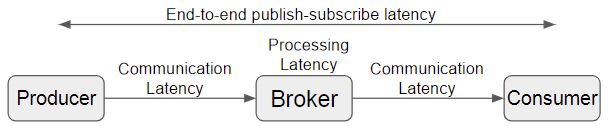
\includegraphics[width=0.75\columnwidth]{figures/epulsar/e2e_latency_breakdown.JPG}
\label{fig:e2e_latency_breakdown}
\caption{Breakdown of end-to-end message delivery latency for a producer-consumer pair.}
\end{figure}
As shown in \cref{fig:e2e_latency_breakdown}, the end-to-end message delivery latency is made up of the communication latency between the producer and serving broker, the latency of handling the message on the broker (potentially persisting it on durable storage in the case of a persistence topic), and the communication latency from the broker to the consumer. The sum of all these component latencies needs to be below the latency threshold. This constraint needs to be satisfied for each producer-consumer pair of the given topic, which may have disparate connectivity to the serving broker compared to other producer-consumer pairs. Hence the broker selection policy needs to select a broker for hosting a topic that is (a) in network proximity to the clients of the topic to ensure low communication latency, and (b) is not overloaded to ensure low processing latency.

\subsubsection{Violation Detection Policy}
The violation Detection Policy of \epulsar{} is used to check whether an existing topic in the publish-subscribe system has its end-to-end message delivery latency constraint violated. This computation is done for each topic independently. Since publisher and subscriber clients of a topic can be connected at different points in the network topology, the worst-case message delivery latency is incurred for the publisher-subscriber pair that are the furthest from the broker. Thus, all possible publisher-subscriber pairs have to be analyzed to check for violations.
\par The worst-case message delivery latency for a topic is the sum of the maximum network latency from any publisher to the broker, the maximum network latency from the broker to any subscriber, and the per-message processing latency on the broker. The worst-case message delivery latency of a topic is compared against the topic-specific threshold, and if the observed latency exceeds the threshold, a violation is detected, and a reconfiguration action is triggered.
%The first two components is calculated using the clients' network coordinates, while the processing latency is estimated by using a profile of the broker's data-plane through offline profiling.
\subsection{Use of Proposed Mechanisms in Control Plane}
\epulsar{}'s control plane utilizes the Network Proximity mechanism to estimate the worst-case message delivery latency for a given topic. This mechanism is able to estimate the communication component of the message delivery latency, while \epulsar{} relies on the an offline profile of its broker for estimating the processing latency. This mechanism is used both for determining whether a particular candidate broker will be able to satisfy the worst-case message delivery latency constraint, given the network proximity information between the clients and the candidate broker. The Network Proximity mechanism is also used for detecting a violation of the worst-case message delivery latency constraint. The clients' network proximity to the current serving broker is used to compute the observed worst-case message delivery latency, which is then compared against the topic-specific threshold.

\section{End-to-End Latency Estimation using Network Proximity Mechanism}
\label{sec:epulsar_nw_prox}
\begin{figure}[h]
\centering
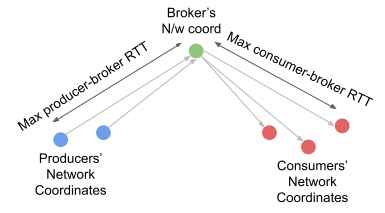
\includegraphics[width=0.75\columnwidth]{figures/epulsar/nw_coord_latency.png}
\label{fig:nw_coord_latency}
\caption{Illustration of the use of network coordinates for computing the worst-case message delivery latency for a given topic. Network coordinates can be used to compute the communication component of the message delivery latency. Since all publisher-subscriber pairs communicate via the broker, computing the maximum network latency from the publishers to the broker and that from the broker to the subscribers suffices to compute the worst-case communication latency across all publisher-subscribe pairs.}
\end{figure}
\subsection{Deployment of Network Coordinate Agents}
To be able to estimate the network latency between every client and broker pair requires that all of those components have an associated network coordinate, such that by computing the Euclidean distance between the coordinates of two nodes, one can compute the communication latency between them. \epulsar{} co-located one instance of the Network Coordinate Agent with each broker, such that the network coordinate of the agent is the same as that of the broker. Clients that are not mobile (e.g., connected to a wired network) also run a Network Coordinate Agent instance and use the agent's coordinate as their own. To handle mobile clients, \epulsar{} relies on a network of Edge Gateways that each run a Network Coordinate Agent. Each client discovers the current serving Edge Gateway using a DNS-like discovery mechanism, records the network round-trip time to the Gateway and computes its own network coordinate from the network coordinate of the Gateway and the measured network round-trip time. The deployment is illustrated in \cref{fig:epulsar_nc_deployment}. The network coordinate of all these system entities is utilized by the broker selection and violation detection policies for estimating the communication component of the end-to-end message delivery latency. 
\begin{figure}[h]
\centering
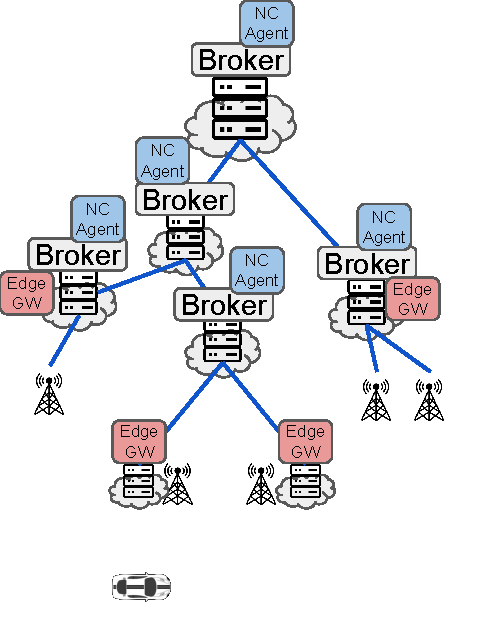
\includegraphics[width=0.5\columnwidth]{figures/epulsar/nc_agent_deployment}
\label{fig:epulsar_nc_deployment}
\caption{Illustration of the deployment of network coordinate agents in \epulsar{}.}
\end{figure}

\begin{table}[t]
	\center
	%\begin{adjustbox}{width=0.8\columnwidth,center}
		\begin{tabular}{ |c|c| } 
			\hline
			\textbf{Notation} & \textbf{Definition}\\ 
			\hline
			$t$ & topic\\
			$P\left( t \right)$ & producers of topic $t$\\
			$C\left( t \right)$ & consumers of topic $t$\\
			$L_{th}\left( t \right)$ & end-to-end latency constraint for topic $t$\\
			$P\left[ t \right]$ & broker hosting topic $t$\\
			$NC\left( i \right)$ & network coordinate of entity $i$\\
			$\overline{NC}\left( I \right)$ & centroid network coordinate of entities in $I$\\
			$d\left( nc_1, nc_2 \right)$ & distance between network coordinates\\
			$W\left( t \right)$ & Deviation of client NC from centroids of topic $t$\\
			$E\left( t \right)$ & Worst-case end-to-end latency for topic $t$\\
			$PROC \left( t \right)$ & Processing latency at broker for topic $t$\\
			\hline
		\end{tabular}
	%\end{adjustbox}
	\caption{Notations used.\todo{Fix the notations based on the actual equations used.}}\label{table:notations}
\end{table}

\subsection{Broker Selection Policy}
The set of publishers and subscribers for a topic $t$ is denoted by $P \left( t \right)$ and $C \left( t \right)$ respectively. The worst-case message delivery latency for topic $t$ is represented as shown in \cref{eq:e2e_latency}.
\begin{equation}
\max\limits_{p \in P\left( t \right)} d \left( NC \left( p\right), NC \left( b\right) \right) + \max\limits_{c \in C\left( t \right)} d \left( NC \left( c\right), NC \left( b\right)\right) + PROC \left( t \right)
\label{eq:e2e_latency}
\end{equation}

\begin{algorithm}
\caption{Broker selection policy algorithm. Inputs are $T$ (set of topics to place on brokers) and $M$ (monitoring data)}\label{broker_sel_algo}
\begin{algorithmic}[1]
\Procedure{SelectBroker}{$T, P, M$}
\State $F \gets dict\left(\right)$
\For{$t \in T$}
    \State $F \left[ t \right] \gets get\_feasible\_brokers\_by\_latency \left( t , M\right)$
\EndFor
\State $\text{sort } T \text{ by increasing } |F \left[ t \right]|$
\For {$t \in T$}
    \For {$b_{cand} \in F \left[ t \right]$}
        \If{$can\_host \left( b_{cand}, t, P, M\right)$} \Comment{no broker overload}
            \State $P \left[ t \right] \gets b_{cand}$
            \State break
        \EndIf
    \EndFor
\EndFor
\State $\text{return } P$
\EndProcedure
\end{algorithmic}
\end{algorithm}

- \todo{Add equations and algorithm for broker selection}

\subsection{Violation Detection Policy}
\todo{Add content about the violation detection policy}
\begin{algorithm}
\caption{Violation Detection Policy algorithm. \todo{Add inputs to the algo}}\label{viol_detection_algo}
\begin{algorithmic}[1]
\Procedure{PerformRepartitioning}{$P_0$, $M$}
\State $R \gets \{\}$ \Comment{set of migration commands}
\State $T_{migr} \gets \{\}$ \Comment{topics to migrate from curr broker}
\For{$t \in P_0.topics$}
    \If{$latency\_violated \left( t \right)$}
        \State $T_{migr} \gets T_{migr} \cup \{ t \}$
    \EndIf
\EndFor

%\State $P \gets PlaceTopics \left( T_{migr}, P_0, M \right)$ 
\State $B_{overload} \gets get\_overloaded\_brokers \left( P_0, M \right)$
\For{$b \in B_{overload}$} \Comment{resource-based detection}
    \State $T_b \gets get\_topics\_to\_migrate\left(b, P_0, M\right)$
    \State $T_{migr} \gets T_{migr} \cup T_b$
\EndFor

\State $P \gets PlaceTopics \left( T_{migr}, P_0, M \right)$ 

\State $R \gets \{\}$ \Comment{set of re-partitioning commands}
\For {$t \in P_0.topics$}
    \If {$P\left[ t \right] \neq P_0 \left[ t \right]$}
        \State $R \gets R \cup \{ \left( t, P_0 \left[ t \right], P \left[ t \right]\right) \}$
    \EndIf
\EndFor
\State $execute\_reconfigs \left( R \right)$ 
\EndProcedure
\end{algorithmic}
\end{algorithm}

\section{Distributed Monitoring in ePulsar}
\label{sec:epulsar_dist_mon}
\subsection{Distribution of Monitoring Components over Infrastructure}
\epulsar{} performs monitoring of the network coordinates of clients and broker as well as the message rate of each topic on the broker that is hosting the topic. Since all the relevant metrics of a given topic are present on the broker itself, it can aggregate the topic's metrics to reduce the amount of data that needs to be sent to the Metrics Store via the wide-area network.

\subsection{Monitoring Data Aggregation Logic}

\epulsar{} reduces the amount of per-topic monitoring data sent to the Metric Store by aggregating the network coordinates of multiple clients. For each topic $t$ that is hosted on broker $b$, we report the following data items through monitoring. \cref{table:notations} provides a summary of notations used.
\begin{itemize}
\item \textbf{Producer and Consumer Centroid.} The producer and consumer centroids provide an approximate location of the network \textit{location} of a topic's clients. We compute the centroid producer coordinate $\overline{NC_P}\left( t \right)$ and centroid consumer coordinate $\overline{NC_C}\left( t \right)$ as follows.
\begin{equation*}
\overline{NC_P}\left( t \right) = \overline{NC} \left( \{ i : i \in P\left( t \right) \} \right)
\end{equation*}
\begin{equation*}
\overline{NC_C}\left( t \right) = \overline{NC} \left( \{ i : i \in C\left( t \right) \} \right)
\end{equation*}
\item \textbf{Maximum Deviation from Centroids.} To cope with the loss of information with centroids, we send the maximum deviation of the clients' coordinates from their corresponding centroid. We denote this as $W \left( t \right)$ and it is computed as shown below.
\begin{equation*}
\max\limits_{p \in P\left( t \right)} d \left( NC \left( p\right), \overline{NC_P}\left( t \right)\right) + \max\limits_{c \in C\left( t \right)} d \left( NC \left( c\right), \overline{NC_C}\left( t \right)\right)
\end{equation*}
\item \textbf{Worst-case End-to-end Latency.} For each topic $t$, we compute the worst-case pub-sub latency across all producer-consumer pairs. We denote this as $E \left( t \right)$ and it is computed as follows. 
\begin{equation*}
\max\limits_{p \in P\left( t \right)} d \left( NC \left( p\right), \overline{NC}\left( P\left[ t \right] \right) \right) + \max\limits_{c \in C\left( t \right)} d \left( NC \left( c\right), \overline{NC}\left( P\left[ t \right] \right) \right) 
\end{equation*}
This information is used to determine whether the current broker, denoted by $P\left[ t \right]$ is meeting the topic's end-to-end pub-sub latency threshold.
\end{itemize}

\par One key point to take note of is that the volume of per-topic monitoring data generated is independent of the number of clients using that topic. Given the high heterogeneity of broker and client network locations in a geo-distributed setting, this aggregation technique significantly reduces monitoring data traffic. By contrast, a naive approach which records the network coordinates of all clients would incur network traffic proportional to the number of clients of each topic.

- \todo{Add equations about the aggregation functions}
- \todo{Describe how the above policies are updated in the presence of distributed monitoring}
\begin{equation}
W \left( t, b\right) = d \left( \overline{NC_P} \left( t \right), NC \left( b \right) \right) + d \left( \overline{NC_C} \left( t \right), NC \left( b \right) \right) + W \left( t \right) 
\vspace{-0.05in}
\end{equation}

\section{Topic Migration}
\todo{Where should we add content about Topic Migrations?}

\section{Implementation of \epulsar{}}
\label{sec:epulsar_impl}
\epulsar{} is implemented by extending Apache Pulsar v2.2.1. We chose Pulsar as the base system because of the strong data-plane semantics that it offers and topic migrations are much more agile than in Apache Kafka. However, Pulsar, like Kafka, is designed for datacenters and bundles topics together for monitoring and placement on brokers. This bundling is done for reducing the amount of metadata is has to maintain. \epulsar{} needs to independently manage each topic, and hence, we restrict the maximum number of topics in a bundle to be 1. When more than one topics are mapped to a bundle, it results in the bundle being split into two new bundles, each with one topic. By keeping the concept of bundles from Pulsar, \epulsar{} is able to re-use the bundle-centric monitoring and broker selection in Pulsar, while still achieving per-topic independent management.
\par The control-plane policies of broker selection and violation detection are implemented in the Load Manager module of Pulsar. We replace the off-the-shelf Load Manager of Pulsar, which aims at even distribution of workload and prevention of hotspots, with an edge-centric implementation that takes communication latency into account as well. \epulsar{} inherits from Pulsar the use of a ZooKeeper instance as the Metrics Store, which is also used for storing configuration information about the system, e.g., topic ownership for each broker, cluster membership, etc. The monitoring data is queried by the Load Manager module periodically every 5 seconds to detect violations and compute better brokers for topics which are undergoing latency constraint violation.

\par Brokers in \epulsar{} run at Edge sites along with cloud datacenters. The control-plane component of Pulsar, i.e., Load Manager, runs in one of the brokers at a time, which serves as the Leader broker of the cluster. In \epulsar{} the Leader broker is forced to be one which is deployed in a datacenter for better availability. Hence, \epulsar{} has a centralized control-plane located in a cloud datacenter. The ZooKeeper instance which serves as the Metrics Store is co-located in the same datacenter as the Leader broker running the Load Manager module. Clients connect to the publish-subscribe infrastructure via various access media, e.g., cellular (4G LTE), WiFi or wired networks. All entities in the publish-subscribe system, including brokers and clients periodically (every 5 seconds) query their network coordinate, either from the Network Coordinate Agent co-located with them (in the case of brokers and static clients) or from the serving Edge Gateway (in the case of mobile clients).

\section{Evaluations}
\label{sec:epulsar_evals}
In this section, we present a set of evaluations to demonstrate the efficacy of the proposed mechanisms in enabling an edge-centric latency-aware control-plane for a geo-distributed publish-subscribe system \epulsar{}. Specifically, we aim to prove the following hypotheses through experimentation.
\begin{enumerate}
\item Incorporating network proximity information in the broker selection policy allows the satisfaction of per-topic latency constraints. Aggregation of client network coordinates does not impair the quality of the broker selection decision.
\item Distributed monitoring results in monitoring overhead reduction.
\item \epulsar{} is able to meet E2E latency %threshold 
constraints for exemplar applications.
\end{enumerate}
We verify the above hypotheses using two main methods: (1) Microbenchmarks that analyze different parts of \epulsar's architecture in isolation. (2) End-to-end evaluations of the UAV Swarm application scenario consisting of realistic infrastructure topology and client workload.

\subsection{Evaluation Scenario}
\label{sec:epulsar_eval_scenario}
We evaluate \epulsar{} under realistic infrastructure and subscription patterns. We consider the following evaluation scenario from which we design microbenchmarks and end-to-end experiments.
\par A UAV swarm consists of multiple drones that move together to accomplish a given task. The swarm contains a leader UAV and the rest of the UAVs are followers. Each swarm follows a Random Waypoint mobility model \cite{rwp}.\\
\textbf{Subscription Pattern. } The leader UAV sends movement commands to the followers through a topic called \textit{follow\_leader}. The followers communicate information extracted from onboard sensors to the leader via a topic \textit{sensor\_data}. The E2E pub-sub latency constraint is set at 40 ms.\\
\textbf{Infrastructure. } We consider a city-wide cellular network equipped with edge resources, where UAVs use LTE as the communication medium. We assume that the city is divided into multiple \textit{Mobile Edge Computing (MEC)} zones, each with a single edge site. The locations of the edge sites is determined via k-means clustering on the cell tower locations \cite{wang2019edge} of Atlanta~\cite{cellmapper}. The edge sites communicate with each other via a city-level switch, with inter-site RTT of 30 ms. Each edge site hosts a broker and an Edge Gateway. Each client is directly connected to the edge site corresponding to its current location based on k-means clustering. Since clients are mobile, they query NC from the respective sites they are directly connected to. The broker running the Load Manager component and the ZooKeeper instance is hosted in the cloud with a one-way latency of 40 ms to any edge site.

\subsection{Evaluation Platform}
The evaluation scenarios described in \cref{sec:epulsar_eval_scenario} pose the following requirements to be satisfied by the evaluation platform: (i) support a heterogeneous network topology, (ii) allow emulation of unmodified software components (\epulsar{} entities and clients), and (iii) emulate device mobility. To satisfy these requirements, we use the \textit{Containernet} \cite{containernet} evaluation platform, which has also been used by previous edge computing research \cite{rothenberg2020intent,fiandrino2019openleon}. Containernet uses Docker containers as hosts (allowing use of unmodified software entities) in network topologies emulated using Open vSwitch. %\todo{Kishore: reworded next sentence.  Please check. Harshit : Looks good.} 
We set custom latencies on the network links using the Linux tool \emph{tc} (to support heterogeneous topologies), and remove/create network links on the fly (to emulate device mobility). 
The emulated infrastructure is deployed on an Ubuntu 16.04 VM with 48 CPU cores and 64 GB RAM. We use Docker's resource reservation to allocate dedicated resources to each container and minimize performance interference.


\subsection{Evaluation of Broker Selection Policy}
In this section, we evaluate the effectiveness of \epulsar{}'s broker selection policy to meet E2E message delivery latency guarantees for realistic infrastructure topologies and client subscription patterns. We compare the proposed policy against the following two baselines.
\begin{itemize}
\item \textbf{AllPairs}. Same as \epulsar, but instead of clients' NC  centroids, \textbf{AllPairs} takes the NC of each individual client and computes the expected E2E latency for each producer-consumer pair. A broker is chosen only if the worst-case E2E latency falls below the threshold.
\item \textbf{Pulsar}. As mentioned in \Cref{sec:stateoftheart}, Pulsar offers well-developed data-plane semantics which are appropriate for the target applications for the edge. Therefore, we choose Pulsar as the other baseline. Pulsar uses consistent hashing to compute the hash for a topic name. The output space of the hash function is divided among all brokers uniformly. The topic is assigned to the broker whose hash-space partition contains the topic's hash.
\end{itemize}

For the representative application scenario mentioned in \cref{sec:epulsar_eval_scenario}, we generate infrastructure topologies with varying degrees of geo-distribution by varying the number of MEC zones in the metropolitan area. For each such topology, we first emulate the infrastructure of the given topology using Containernet. After allowing the NC agents in brokers and clients to stabilize for 10 minutes, we query each agent's coordinate. The querying is done once per topology. Using the coordinates of all nodes in the topology, we can then estimate the E2E delay for any producer-consumer pair of a topic given the location of the clients and the broker hosting that topic. Based on the application scenario's subscription pattern, we determine the clients for each topic and place them on the nodes of the generated topology. 

The network coordinates of the producers and consumers for each topic serve as the input to the broker selection policy. We analyze the result of selection policy in terms of the E2E latency and violation ratio. Violation ratio represents the fraction of producer-consumer pairs for whom the latency threshold is violated. In the experiments, we consider 1000 different random permutations of client placement and topic subscriptions.  The intent is to have a large coverage of possibilities wherein clients could be located in different geographical areas and/or could be subscribing to different sets of topics.

\par We vary the number of MEC zones in the simulated metro area and distribute 16 UAV swarms in the city. Each swarm comprises 8 UAVs, with one of them serving as the leader. UAVs follow the subscription pattern described in \cref{sec:epulsar_eval_scenario}. 
\begin{figure}[ht]
\begin{subfigure}{.45\columnwidth}
  \centering
    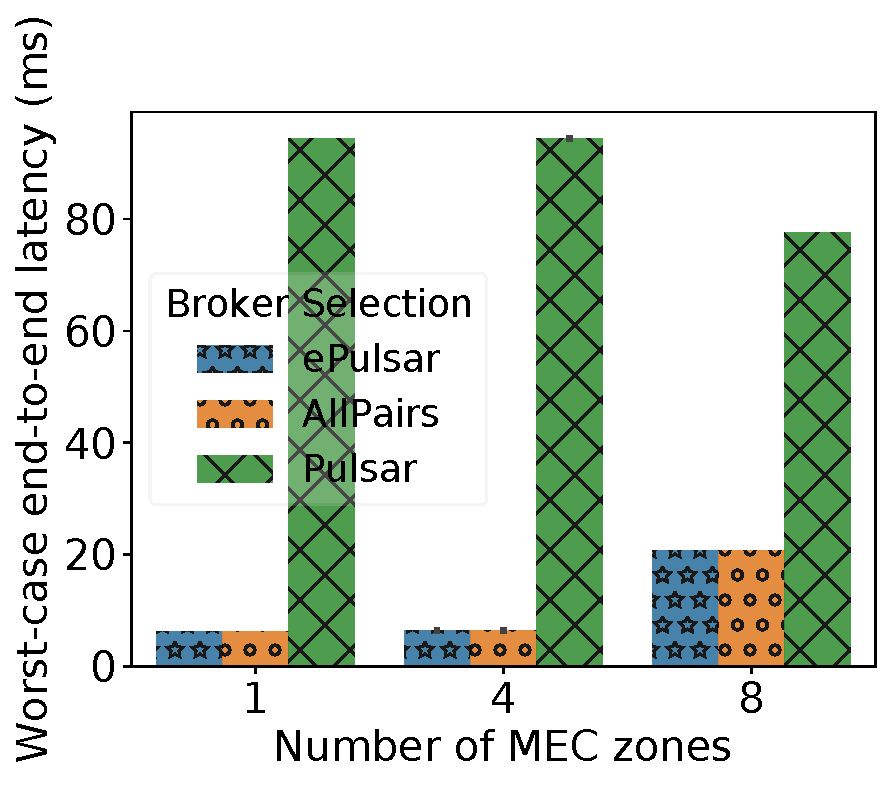
\includegraphics[width=\columnwidth]{figures/epulsar/evals/latency.pdf}
    \caption{Worst-case E2E latency}
    \label{fig:brokersel_uav_latency}
\end{subfigure}
\begin{subfigure}{.45\columnwidth}
  \centering
    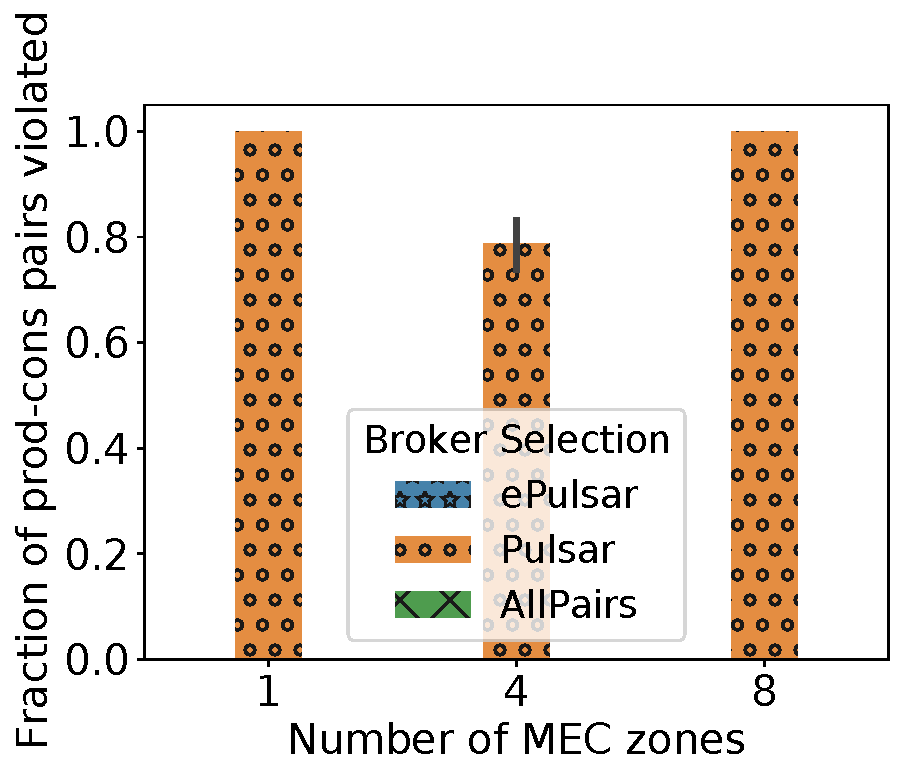
\includegraphics[width=\columnwidth]{figures/epulsar/evals/violation_ratio.pdf}
    \caption{Violation Ratio.}
    \label{fig:brokersel_uav_viol}
\end{subfigure}
\caption{Analysis of broker selection policy for UAV swarm application scenario.}
\label{fig:broker_sel_uav}
\end{figure}
\cref{fig:brokersel_uav_latency,fig:brokersel_uav_viol} show the worst-case E2E latency and violation ratio over all producer-consumer pairs. Since \epulsar{} performs latency-aware topic partitioning, the worst-case latency remains under the threshold, resulting in no violations even when the number of MEC zones is increased. 
The results in this subsection, for both application scenarios, validate the first hypothesis that the incorporation of network coordinates information in the broker selection policy improves the satisfaction of end-to-end message delivery latency constraint. Furthermore, the comparison with the AllPairs policy shows that the aggregation of clients' network coordinates as centroids does not result in poor broker selection with respect to meeting E2E latency constraints.

\subsection{Evaluation of Distributed Monitoring}
We evaluate the savings in monitoring traffic by aggregating per-topic client NCs at the serving broker before reporting them to the Metrics Store. This traffic is sent continuously through the WAN and impacts scalability of the system, hence we consider aggregate monitoring traffic rate as the metric-of-interest. We focus our evaluation on a single broker hosting topics with multiple clients - as the behavior is independent of other brokers. We vary the number of topics hosted on the broker and the number of clients connected to each topic.
\begin{figure}[ht]
% Taken from exp ID ZKDELAY_2021-01-18-00-43-28
  \centering
  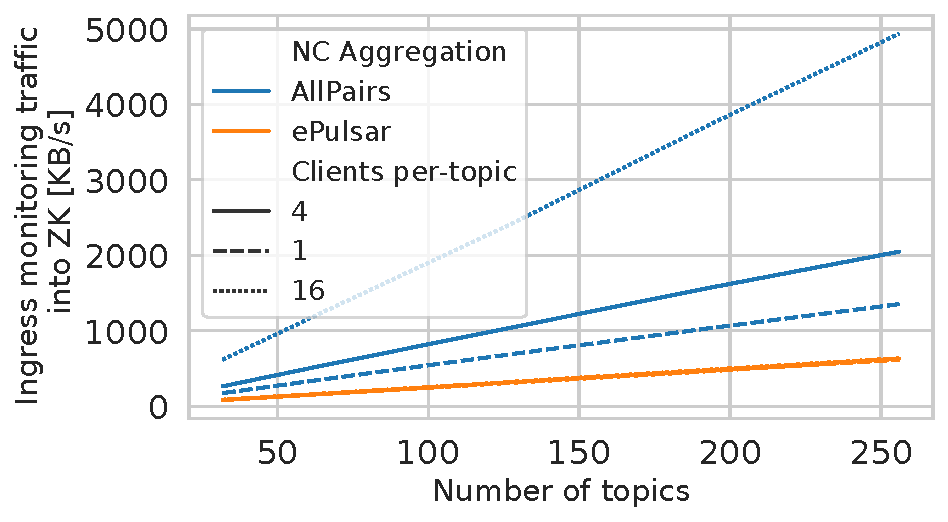
\includegraphics[width=0.9\linewidth]{figures/epulsar/evals/zk_traffic_rate__.pdf}  
  \caption{Monitoring traffic rate under varying number of topics and clients per topic. \epulsar's NC aggregation results in considerable savings over naive AllPairs.}
    \label{fig:zk_traffic_rate}
\end{figure}

\cref{fig:zk_traffic_rate} shows the data rate of monitoring traffic sent to the Metrics Store. An increasing number of topics results in higher data rate. The rate of increase is higher without centroid aggregation (AllPairs policy) and also with more clients per topic. \epulsar's aggregation, however, causes data rate to be independent of the number of clients - since a constant amount of data is sent to the Metrics Store per topic. These results validate the second hypothesis that aggregating clients' network coordinates as centroids results in reducing the monitoring overhead.

\subsection{End-to-End Evaluation}
In this section, we evaluate \epulsar's ability to respect E2E latency constraints of the exemplar UAV Swarm application, and validate the third hypothesis. The metric we use for the evaluation is E2E message delivery latency -- i.e., the elapsed time between a client publishing on a topic and the receipt of the published message by all the clients subscribing to that topic.

\begin{figure*}[!t]
    \centering
    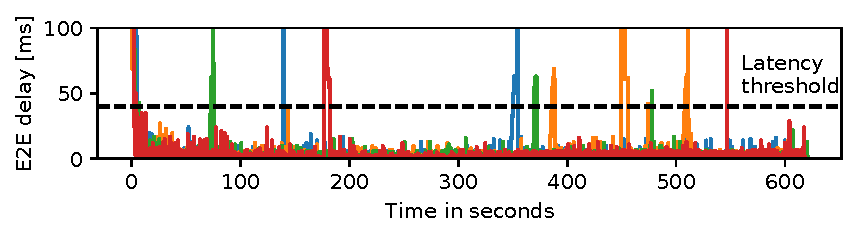
\includegraphics[width=0.7\textwidth]{figures/epulsar/evals/e2e_delays_swarm_combined.pdf}
    \caption{E2E latencies experienced by the 8 independent drone swarms for their respective representative topic over time. Latency violations (transient spikes) are observed when a swarm moves from one MEC zone to another.  For a brief period, the latency remains higher than the threshold. \epulsar's topic migration brings the latency back under the threshold.}
    \label{fig:e2e_drone_swarm_aggr}
\end{figure*}

We consider the infrastructure topology described in \cref{sec:epulsar_eval_scenario} with 4 MEC zones and emulate using Containernet. We emulate each UAV swarm as an independent container where the mobility of all of the members of the swarm are identical. In the emulated network topology, each zone consists of a network switch to which the broker and the Edge Gateway connect. We create a link between the swarm's container and the switch corresponding to the swarm's current MEC zone. When a swarm moves into a new zone, the link to the previous zone's switch is removed and a link to the new zone's switch is created. We emulate 8 independent swarms, each with 8 UAVs, following the Random Waypoint mobility model in the city at a relatively high speed of 50 meters/sec\footnote{We use such a high speed to trigger several mobility-driven topic migrations during the experiment.}. Both leader and followers generate 200 msgs/sec each of size 1 KB \cite{yang2018telecom}. We perform this experiment for 10 minutes.
\par We show the E2E latency of a single representative topic from each swarm in \cref{fig:e2e_drone_swarm_aggr}\footnote{To avoid cluttering the figure, we do not show all the topics of each swarm since their behavior is identical.}.
For each swarm. the E2E latency remains under the latency threshold  (40 ms) for most of the experiment duration. Transient violations of latency threshold occur when a swarm moves into a different MEC zone than the one currently hosting the swarm's topics. \epulsar{}'s monitoring module detects such violations and triggers migration of the swarm's topics to the broker at the new MEC zone, after which the E2E latency returns back under the latency threshold.

\section{Conclusion}
\label{sec:epulsar_conclusion}